\providecommand{\main}{..}
\documentclass[\main/master.tex]{subfiles}
\begin{document}
\chapter{methods and results}\label{chp:example-2}
\section{System design}
\subsection{Vacuum Quality}
\subsubsection{Leak Rate}
At any gas system, some gas would slowly leak over time and increase the pressure if not pumped out. The leak rate $Q_L$ is not a function of time but volume, and resuls in a sustained increase of pressure P over time.
\begin{equation}
Q_L = \frac{\Delta P\cdot V}{\Delta t}  \label{eqn:energy-mass-equivalence-relation}
\end{equation}
The leak rate could also prevant the system from reaching initial low pressure (at some point the leakage would be equal to the pumping rate).
\par
There is also diffusion rate of gas molecules, such as helium, which is insignifant when pressure is above $10^{-9}$ [Torr] (vacuum lower than high vacuum). 

\subsubsection{Outgassing}
At low pressures, there are more gas molecules adsorbed on the chamber surface than floating in the chamber. When pressure is below vapour pressure theres a desorption of gas molecules (primarily water) from the material.
\par
Outgassing is the desorption rate $Q_{des}$ over time increasing the pressure. The desorption rate depends on the surface area and the desorption density $q_{des}$ which is area specific. 
\begin{equation}
Q_{des} = q_{des}\cdot A\cdot\frac{t_0}{t}  \label{eqn:energy-mass-equivalence-relation}
\end{equation}
The desorption rate produces a gas yield that declines over time. It could be assumed that after a given time $t>t_0$ the increase is liniar over time, typicaly $t_0$ assumed to be one hour.
\par
Outgassing is minimized by selection of low vapor pressures materials such as stainless steel and glass. Since water is a significant source of outgassing, it is usually minimize by baking the chamber at high tempertures while the pump is running.
\subsubsection{Vacuum Chambers}
Vaccuum chambers are metalic chambers connected to a vacuum pump with pressure lower than the atmospheric pressure. The main limitations to vacuum quality maintenance are leakage from the outside through the chamber and outgassing inside the chamber.
\par
Leaks and outgassing both increases the pressure (lowering the vacuum) at a constant rate over time. Usually, in order to keep equilibrium, the leaks and outgassing overcome by having a constant pump rate (vacuum pump working).   
\begin{equation}
Q_P = Q_L + Q_{des}  \label{eqn:vacuum_equilibrium}
\end{equation}
In this experiment due to the relatively large size and uniqe shape of the measurement equipment, the vacuum chamber is having both a large leak and outgassing over time. The sensetivity of the measuerment did not allow having the pump working, causing pressure increase over time.
\par 
In order to minimize the pressure increase over time vacuum chamber was built using CF Style Vacuum Components, designed for ultra high vacuum. The meausrement system inside chamber was designed to function after being exposed to high tempertures while baking.
\subsection{Chamber Design}

Chamber and torsional pendulum design was carried out using Solid Works. The chamber build is two cylindrical tubes placed on each other with three view ports in front. The chamber has a 5-way which is connected to the vacuum engine and gauge. The torsional pendulum is placed inside the chamber. Vacuum engine is connected to chamber through a valve, measurement is made when valve closed and engine off, to prevent rotation noise.




\begin{figure}[htbp]
	\centering
	\fbox{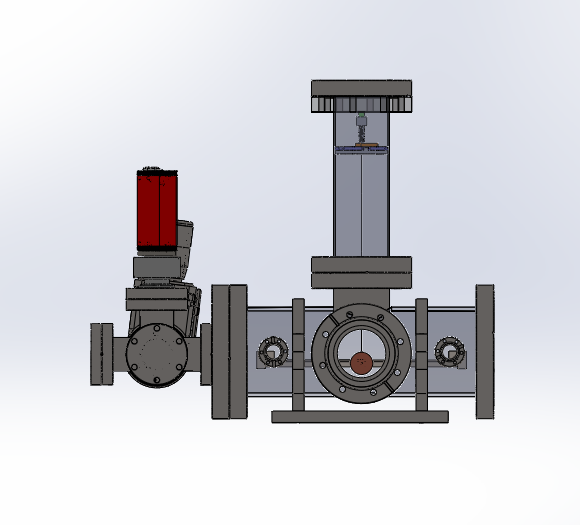
\includegraphics[scale=0.3]{\main/images/4 - methods and results/total_chamber.png}}
	\caption[mount]{mount}
	\label{fig:mount}
\end{figure}
The the pendulum mount is adjustable, enabling to adjust the hight of pendulum, so it would be in front of viewports accurately. The upper tube of chamber is soldered with a base to which the pendulum mount is connected. The angle of torsion is measured using a mirror connected in front of the pendulum. In order to balance the pendulum so the mirror would not have an initial tilt, center of mass needs to be adjusted. The center of mass is adjusted using a mass from the back, to balance the mirror weight.

\begin{figure}[htbp]
	\centering
	\fbox{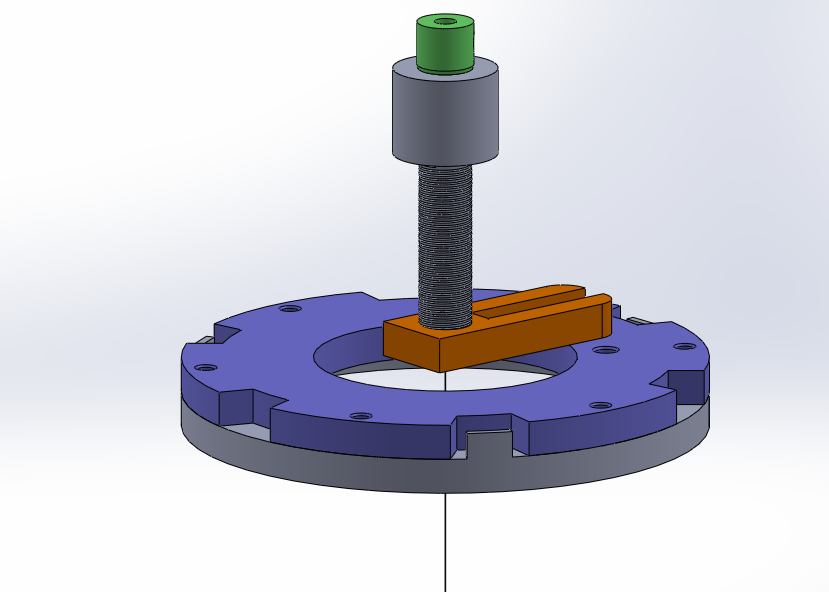
\includegraphics[scale=0.25]{\main/images/4 - methods and results/mount.png}}
	\caption[mount]{mount}
	\label{fig:mount}
\end{figure}




\end{document}